%%%%%%%%%%%%%%%%%%%%%%%%%%%%%%%%%%%%%%%%%
% Simple Sectioned Essay Template
% LaTeX Template
%
% This template has been downloaded from:
% http://www.latextemplates.com
%
% Note:
% The \lipsum[#] commands throughout this template generate dummy text
% to fill the template out. These commands should all be removed when 
% writing essay content.
%
%%%%%%%%%%%%%%%%%%%%%%%%%%%%%%%%%%%%%%%%%

%----------------------------------------------------------------------------------------
%	PACKAGES AND OTHER DOCUMENT CONFIGURATIONS
%----------------------------------------------------------------------------------------

\documentclass[12pt]{article} % Default font size is 12pt, it can be changed here

\usepackage{geometry} % Required to change the page size to A4
\geometry{a4paper} % Set the page size to be A4 as opposed to the default US Letter
\usepackage[UTF8]{ctex}
\usepackage{graphicx} % Required for including pictures
\usepackage{amsmath}
\usepackage{float} % Allows putting an [H] in \begin{figure} to specify the exact location of the figure
\usepackage{wrapfig} % Allows in-line images such as the example fish picture
\usepackage{lipsum} % Used for inserting dummy 'Lorem ipsum' text into the template
\usepackage{url}
\linespread{1.2} % Line spacing
\renewcommand\thesection{\Roman{section}}
%\setlength\parindent{0pt} % Uncomment to remove all indentation from paragraphs

\graphicspath{{Pictures/}} % Specifies the directory where pictures are stored

\begin{document}

%----------------------------------------------------------------------------------------
%	TITLE PAGE
%----------------------------------------------------------------------------------------

\begin{titlepage}

\newcommand{\HRule}{\rule{\linewidth}{0.5mm}} % Defines a new command for the horizontal lines, change thickness here

\center % Center everything on the page

% Name of your university/college
\textsc{\Large 生物信息学}\\[0.5cm] % Major heading such as course name
\textsc{\large 课程报告}\\[0.5cm] % Minor heading such as course title

\HRule \\[0.4cm]
{ \huge \bfseries 基因测序技术发展综述}\\[0.4cm] % Title of your document
\HRule \\[1.5cm]

\begin{minipage}{0.4\textwidth}
\begin{flushleft} \large
\emph{作者:} 
黄俊凯% Your name
\end{flushleft}
\end{minipage}
~
\begin{minipage}{0.4\textwidth}
\begin{flushright} \large
\emph{导师:} 
徐永东% Supervisor's Name
\end{flushright}
\end{minipage}\\[4cm]


\vfill
\textsc{\large  \textbf{\emph{哈尔滨工业大学(威海)}} }\\[0.5cm] 
{\large  \today}\\[2cm] % Date, change the \today to a set date if you want to be precise

%\includegraphics{Logo}\\[1cm] % Include a department/university logo - this will require the graphicx package

 % Fill the rest of the page with whitespace

\end{titlepage}

%----------------------------------------------------------------------------------------
%	TABLE OF CONTENTS
%----------------------------------------------------------------------------------------

\tableofcontents % Include a table of contents

\newpage % Begins the essay on a new page instead of on the same page as the table of contents 

%----------------------------------------------------------------------------------------
%	INTRODUCTION
%----------------------------------------------------------------------------------------

\section{引言} 
随着生物信息学课程的学习,我逐渐对基因测序技术有了很大的兴趣,因此本次课程报告选择对基因测序技术的发展历史以及相关原理做综述。这不算是一篇严格的文献综述,具体来说,应该是我学习基因测序技术的过程。


我们生而为人,既渺小而又伟大。短短的八千多年,从刀耕火种到现代文明,这不得不说是一个奇迹。而这一切,我认为,都源自于人类对自身以及周围环境的不断探索。而对自身的探索,我们从宏观开始,研究人体,研究器官,研究细胞。但这些宏观生命活动的调控者—基因,我们还知之甚少。可以说,人类开始对基因的研究才是对生命物理本质探讨的开始。而要读懂基因内蕴藏的遗传密码,基因测序技术作为我们的强有力的解码工具,不可或缺。


%------------------------------------------------

\section{第一代测序技术} % Sub-section

基本测序方法包括链终止法和化学降解法,与在这基础之上发展的测序方法一并统称为第一代测序技术。第一代测序技术的特点是测序读长可达1000bp\footnote{ bp(base pair),(生物学)碱基对。},准确性高达99.999\%。正由于高精度的特点,现今一代测序仍然是基因检测的标准,也是对新一代测序结果进行评估验证的主要手段。但实际操作中还是存在不少问题,如放射性核素的污染,操作步骤繁琐、效率低和速度慢等缺点,特别是结果判断的读片过程实在是费时又乏味的工作。


双脱氧终止法和化学降解法自1997年提出并的逐渐完善,无疑是目前公认的二种最通用、最有效的DNA序列分析方法,F.Sanger、A.M.Maxam和 W.Gilbert等人也因此分享了1980年度诺贝尔化学奖\footnote{The Nobel Prize in Chemistry 1980,\url{https://www.nobelprize.org/nobel_prizes/chemistry/laureates/1980/} }。。

%------------------------------------------------

\subsection{链终止法} % Sub-section
链终止法(Chain termination DNA Sequencing),由英国剑桥大学的生物化学家F.Sanger于1977年发明。利用这个技术他成功测定了Φ-X174噬菌体(Phage Φ-X174)的基因组序列\cite{Paper:sanger}。


\subsubsection{原理简介}
在DNA的自我复制过程中,双链DNA在酶的作用下解螺旋,局部变成两条单链。以单链为模板,游离的碱基为材料,遵循碱基互补配对原则,在酶的作用下合成一条和模板互补的新的DNA链。Sanger测序法利用了DNA合成的这个过程,通过高温使双链变成两条单链待测模板,引物标定测序的起始点,再加入酶和游离碱基合成互补DNA序列,而链终止法测序的秘密就在于加入的特殊碱基中。


正常的DNA碱基是四种脱氧核糖核苷酸(dNTP),如果将这个碱基稍加改造,将一个-OH的氧去除,变成-CH2,就变成了一个双脱氧的核糖核苷酸(ddNTP)。如图\ref{fig:sanger},在DNA合成的过程中加上这个ddNTP,由于ddNTP无法和下一个碱基链接,DNA链将无法继续延伸。故在Sanger在体系中的dNTP里掺入了一定比例的ddNTP,使得DNA复制时可以在任意位置随机终止,从而产生长短不一的合成产物。将这些长短不同的片段通过电泳加以区分鉴定,从而解密出序列信息。

\begin{figure}[H] % Example image
	\center{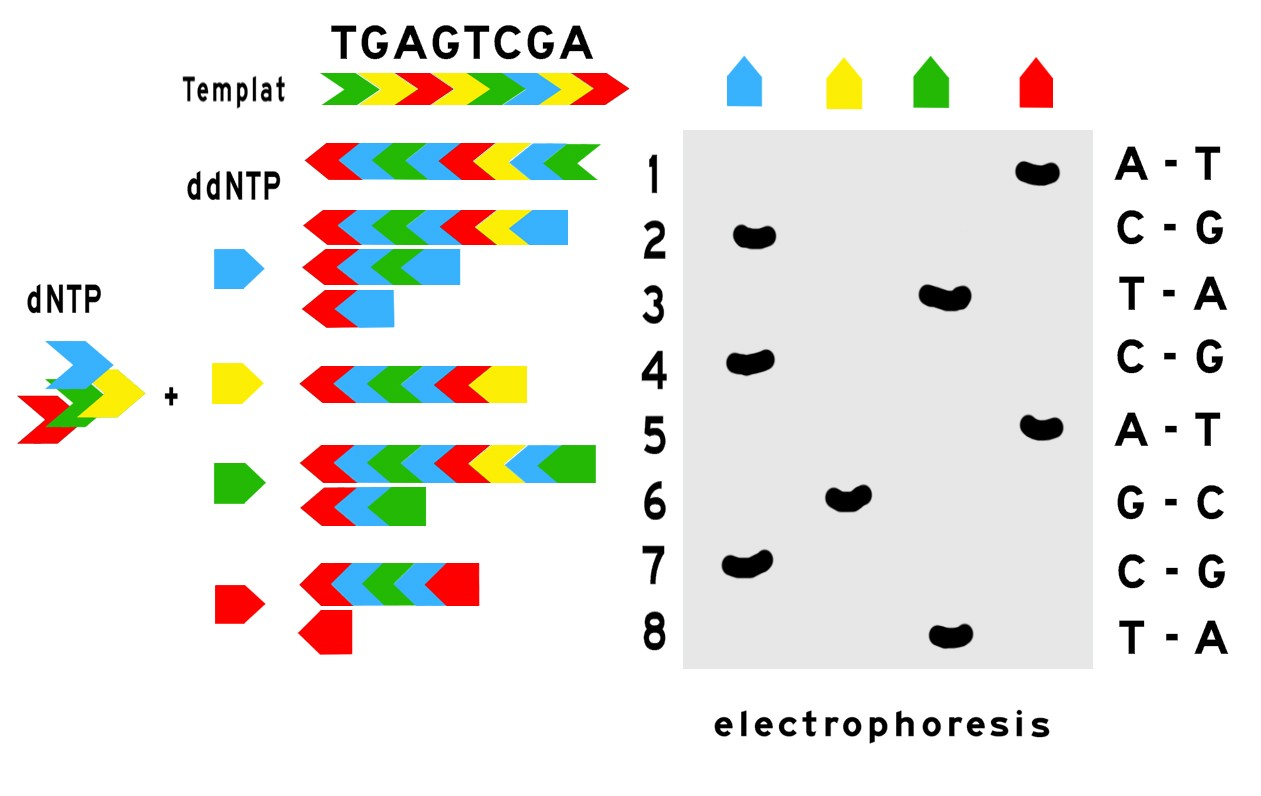
\includegraphics[width=0.5\linewidth]{sanger}}
	\caption{Chain termination DNA Sequencing}
	\label{fig:sanger}
\end{figure}
%------------------------------------------------

\subsection{化学降解法} % Sub-sub-section
化学降解法 (Chemical degradation method),由A.M.Maxam和W.Gilbert于1977年发明。Maxam-Gilbert 化学降解测序法不需要进行酶催化反应,因此不会产生由于酶催化反应而带来的误差,而且对未经克隆的 DNA 片段可以直接测序。化学降解测序法既可以标记 5'-末端,也可以标记 3'-末端。如果从两端分别测定同一条 DNA 链的核苷酸序列,相互参照测定结果,可以得到准确的 DNA 链序列。

%------------------------------------------------

\subsubsection{原理简介} % Sub-sub-section
首先对待测DNA末端进行放射性标记,再通过5组(也可以是4组)相互独立的化学反应分别得到部分降解产物,其中每一组反应特异性地针对某一种或某一类碱基进行切割。因此,产生5组(或4组)不同长度的放射性标记的DNA片段,每组中的每个片段都有放射性标记的共同起点,但长度取决于该组反应针对的碱基在原样品DNA分子上的位置。此后各组反应物通过聚丙烯酰胺凝胶电泳进行分离,通过放射自显影检测末端标记的分子,并直接读取待测DNA片段的核苷酸序列。

\section{第二代测序技术}
 由于测序成本高,通量低等方面的缺点,严重影响了第一代测序技术真正大规模的应用。因此第一代测序技术并不是最理想的测序方法。经过不断的技术开发和改进,以Roche公司的454技术、illumina公司的Solexa,Hiseq技术和ABI公司的Solid技术为标记的第二代测序技术诞生了。 第二代测序也被叫做下一代测序(Next Generation Sequencing,NGS),相比于一代测序,第二代测序技术大大降低了测序成本的同时,还大幅提高了测序速度,并且保持了高准确性,以前完成一个人类基因组的测序需要3年时间,而使用二代测序技术则仅仅需要1周。正是这种改变使得大测序时代的到来真正成为可能。 图\ref{fig:expenschange}是对第一代和第二代测序技术的测序成本进行了一个简单的比较\cite{Paper:Niedringhaus}
\begin{figure}[H] % Example image
	\center{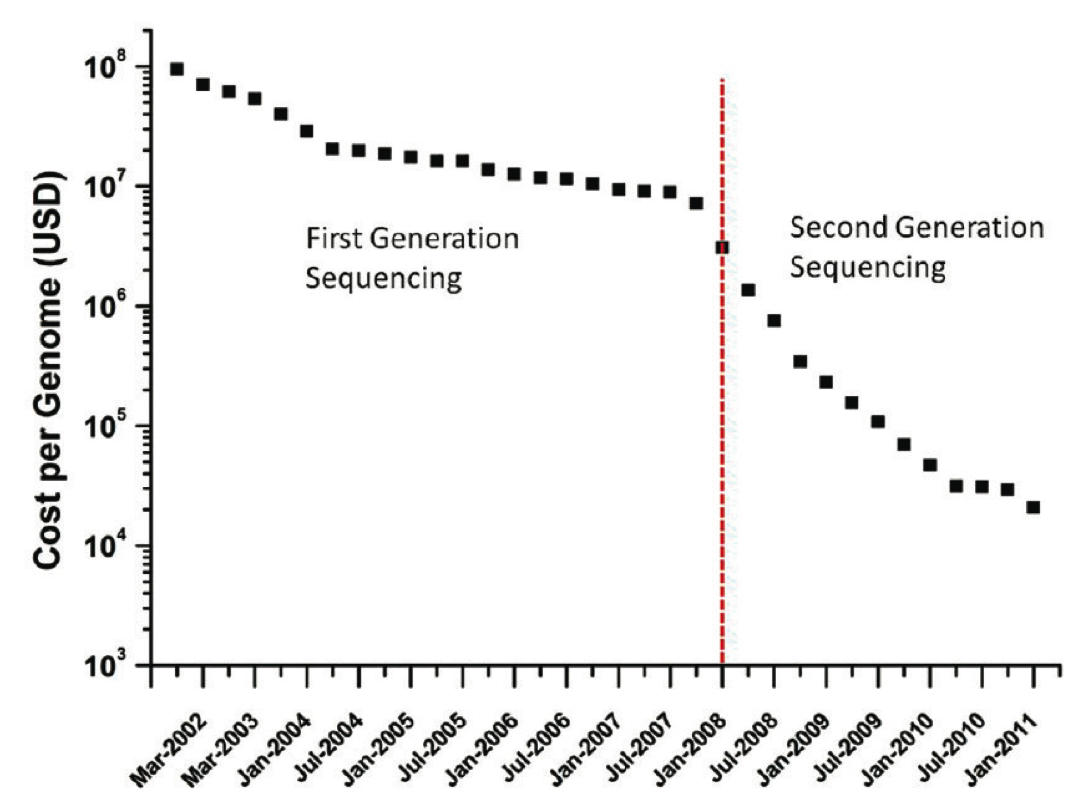
\includegraphics[width=0.5\linewidth]{expenschange}}
	\caption{测序成本变化趋势曲线}
	\label{fig:expenschange}
\end{figure}


不同于一代测序,NGS采用的是边合成边测序的策略,主要的技术路线以Roche公司的454技术、illumina公司的Solexa,Hiseq技术和ABI公司的Solid技术为代表。为了增强测序准确性,需要对同一模板通过PCR扩增多个拷贝来矫正偏差值。因此整个测序分为PCR扩增\footnote{ 一种可以快速复制大量产生相同DNA片段的技术}和测序两个步骤。但是PCR过程会一定程度增加系统的错误率,并且带来的错误具有偏向性,这也是二代技术存在的问题之一。

\subsection{Roche 454}
Roche 454测序系统是第一个商业化运营二代测序技术的平台。采用焦磷酸测序方法和乳液PCR技术,准确率高,读长长,是从头拼接和宏基因组学的理想的选择。不足之处是样品制备较难,难于处理重复和同种碱基多聚区域,成本相对较高。

\subsubsection{原理简介}
\begin{description}
	\item[DNA待测文库构建] \hfill \\
	 如图\ref{fig:rochea}所示,Roche 454测序系统的文件构建方式是利用喷雾法将待测DNA打断成300-800bp长的小片段,并在片段两端加上不同的接头,或将待测DNA变性后用杂交引物进行PCR扩增,连接载体,构建单链DNA文库
	\begin{figure}[H] % Example image
		\center{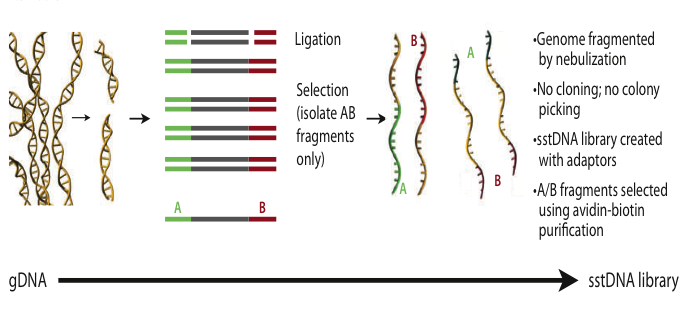
\includegraphics[width=0.5\linewidth]{rochea}}
		\caption{DNA library preparation}
		\label{fig:rochea}
	\end{figure}
	
	\item[Emulsion PCR] \hfill \\
	 DNA扩增过程中,如图\ref{fig:rocheb}所示,Roche 454是将这些单链DNA结合在水油包被的直径约28um的磁珠上,并在其上面孵育、退火。Emulsion PCR最大的特点是可以形成数目庞大的独立反应空间以进行DNA扩增。其关键技术是“注水到油”(水包油),基本过程是在PCR反应前,将包含PCR所有反应成分的水溶液注入到高速旋转的矿物油表面,水溶液瞬间形成无数个被矿物油包裹的小水滴。这些小水滴就构成了独立的PCR反应空间。理想状态下,每个小水滴只含一个DNA模板和一个磁珠。


	这些被小水滴包被的磁珠表面含有与接头互补的DNA序列,因此这些单链DNA序列能够特异地结合在磁珠上。同时孵育体系中含有PCR反应试剂,所以保证了每个与磁珠结合的小片段都能独立进行PCR扩增,并且扩增产物仍可以结合到磁珠上。当反应完成后,可以破坏孵育体系并将带有DNA的磁珠富集下来。进过扩增,每个小片段都将被扩增约100万倍,从而达到下一步测序所要求的DNA量。

	\begin{figure}[H] % Example image
	\center{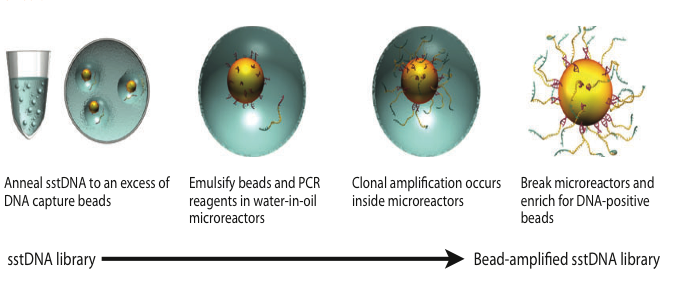
\includegraphics[width=0.5\linewidth]{rocheb}}
	\caption{Emulsion PCR}
	\label{fig:rocheb}
\end{figure}

	\item[测序] \hfill \\ 
	测序前需要先用一种聚合酶和单链结合蛋白处理带有DNA的磁珠,接着将磁珠放在一种PTP平板上。如图\ref{fig:rochec}所示,这种平板上特制有许多直径约为44um的小孔,每个小孔仅能容纳一个磁珠,通过这种方法来固定每个磁珠的位置,以便检测接下来的测序反应过程。  
	
		\begin{figure}[H] % Example image
		\center{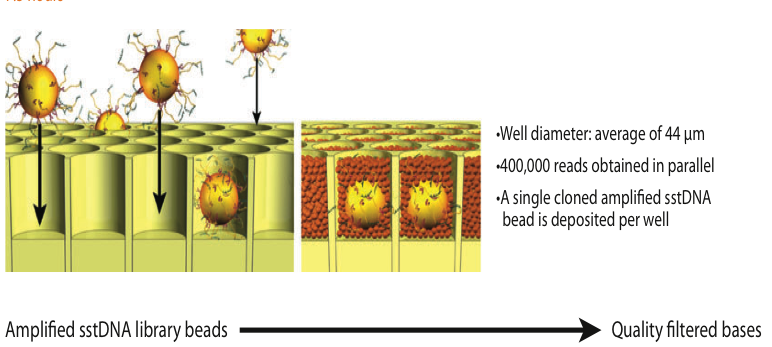
\includegraphics[width=0.5\linewidth]{rochc}}
		\caption{Sequencing}
		\label{fig:rochec}
	\end{figure}
	
	
	测序方法采用焦磷酸测序法\cite{Paper:Mardis, Paper:Shendure, Paper:Mardi},将一种比PTP板上小孔直径更小的磁珠放入小孔中,启动测序反应。测序反应以磁珠上大量扩增出的单链DNA为模板,每次反应加入一种dNTP进行合成反应。如果dNTP能与待测序列配对,则会在合成后释放焦磷酸基团。释放的焦磷酸基团会与反应体系中的ATP硫酸化学酶反应生成ATP。生成的ATP和荧光素酶共同氧化使测序反应中的荧光素分子并发出荧光,同时由PTP板另一侧的CCD照相机记录,最后通过计算机进行光信号处理而获得最终的测序结果。由于每一种dNTP在反应中产生的荧光颜色不同,因此可以根据荧光的颜色来判断被测分子的序列。反应结束后,游离的dNTP会在双磷酸酶的作用下降解ATP,从而导致荧光淬灭,以便使测序反应进入下一个循环。由于454测序技术中,每个测序反应都在PTP板上独立的小孔中进行,因而能大大降低相互间的干扰和测序偏差。
	
	
	454技术最大的优势在于其能获得较长的测序读长,当前454技术的平均读长可达400bp,并且454技术和illumina的Solexa和Hiseq技术不同,它最主要的一个缺点是无法准确测量同聚物的长度,如当序列中存在类似于PolyA的情况时,测序反应会一次加入多个T,而所加入的T的个数只能通过荧光强度推测获得,这就有可能导致结果不准确。也正是由于这一原因,454技术会在测序过程中引入插入和缺失的测序错误。 




\end{description}




\subsection{illumina Solexa}
illumina的Solexa技术是单分子阵列测序,采用桥式PCR扩增,也是当今最有人气的技术,市场份额最高的绝对霸主。其专利核心技术为“DNA簇”和“可逆终止子(Reversible Terminator)”。Solexa\cite{Paper:Mardis,  Paper:Mardi}技术的特别在于速度快(几乎是其他测序技术的100倍)和价格便宜,而其公司提供数据分析配套服务的策略,也帮助illumina公司迅速占领市场,当今已占据超过70\%的市场份额。



\subsubsection{原理简介}

利用超声波把待测的DNA样本打断成小片段,目前除了组装之外和一些其他的特殊要求之外,主要是打断成200-500bp长的序列片段,并在这些小片段的两端添加上不同的接头,构建出单链DNA文库


\begin{description}
	\item[DNA待测文库构建] \hfill \\
	 利用超声波把待测的DNA样本打断成小片段,目前除了组装之外和一些其他的特殊要求之外,主要是打断成200-500bp长的序列片段,并在这些小片段的两端添加上不同的接头,构建出单链DNA文库。
	\item[Flowcell]  \hfill \\
	Flowcell是用于吸附流动DNA片段的槽道,当文库建好后,这些文库中的DNA在通过flowcell的时候会随机附着在flowcell表面的channel上。每个Flowcell有8个channel,每个channel的表面都附有很多接头,这些接头能和建库过程中加在DNA片段两端的接头相互配对(这就是为什么flowcell能吸附建库后的DNA的原因),并能支持DNA在其表面进行桥式PCR的扩增。
	\item[桥式PCR扩增与变性] \hfill \\ 桥式PCR以Flowcell表面所固定的接头为模板,进行桥形扩增,如图\ref{fig:llumina_a}所示。经过不断的扩增和变性循环,最终每个DNA片段都将在各自的位置上集中成束,每一个束都含有单个DNA模板的很多分拷贝,进行这一过程的目的在于实现将碱基的信号强度放大,以达到测序所需的信号要求。
	
	
	\begin{figure}[H] % Example image
		\center{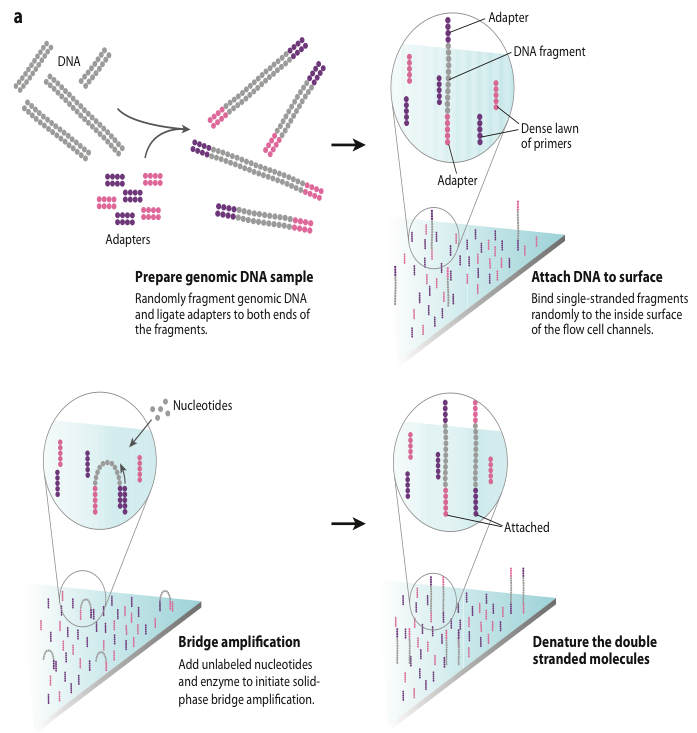
\includegraphics[width=0.7\linewidth]{llumina_a}}
		\caption{桥式PCR扩增与变性}
		\label{fig:llumina_a}
	\end{figure}
	
	\item[测序] \hfill \\
	测序方法采用边合成边测序的方法。向反应体系中同时添加DNA聚合酶、接头引物和带有碱基特异荧光标记的4中dNTP(如同Sanger测序法)。这些dNTP的3’-OH被化学方法所保护,因而每次只能添加一个dNTP。在dNTP被添加到合成链上后,所有未使用的游离dNTP和DNA聚合酶会被洗脱掉。接着,再加入激发荧光所需的缓冲液,用激光激发荧光信号,并有光学设备完成荧光信号的记录,最后利用计算机分析将光学信号转化为测序碱基。这样荧光信号记录完成后,再加入化学试剂淬灭荧光信号并去除dNTP 3’-OH保护基团,以便能进行下一轮的测序反应。
	
				\begin{figure}[H] % Example image
		\center{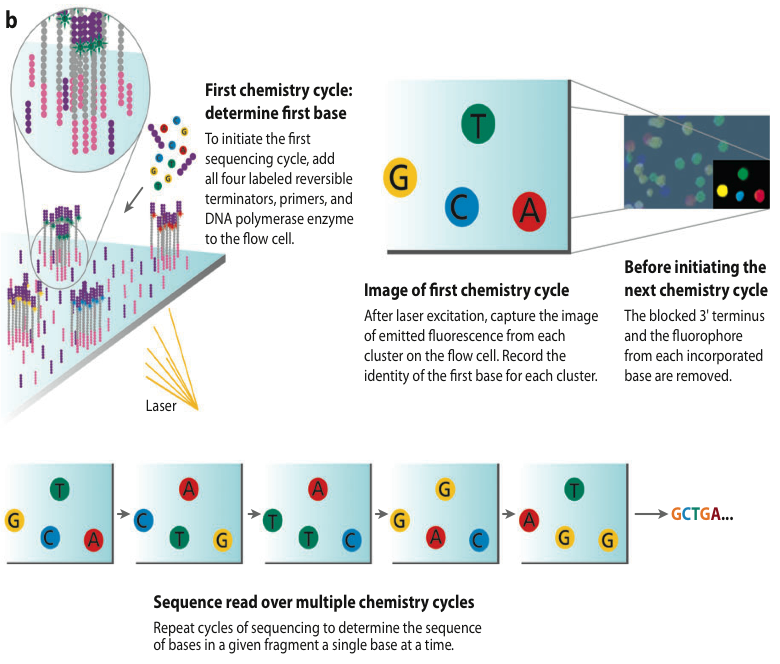
\includegraphics[width=0.7\linewidth]{llumina_b}}
		\caption{测序}
		\label{fig:llumina_b}
	\end{figure}
	
	
	反复循环,即可一个个的同时识别flowcell上固定的所有待测DNA的序列。它的主要测序错误来源是碱基的替换,目前它的测序错误率在1\%-1.5\%之间。
\end{description}







\subsection{ABI Solid}



Solid技术和之前两个合成测序略有不同,是一种连接测序技术。不是单个碱基识别荧光,而是连续的双碱基共同编码,基于连接酶法,即利用DNA连接酶在连接过程之中测序。超高的通量是其一大特色,SOLiD 3系统单次运行可产生50GB的数据,相当于17倍人类基因组覆盖度。准确性、系统可靠性和可扩展性都很好,可是读长太短(25-35bp),运行时间太长。

\subsubsection{原理简介}

\begin{description}
	\item[DNA文库构建] \hfill \\
	片段打断并在片段两端加上测序接头,连接载体,构建单链DNA文库。
	\item[Emulsion PCR] \hfill \\
	 Solid的PCR过程也和454的方法类似,同样采用小水滴emulsion PCR,但这些微珠比起454系统来说则要小得多,只有1um。在扩增的同时对扩增产物的3’端进行修饰,这是为下一步的测序过程作的准备。3’修饰的微珠会被沉积在一块玻片上。在微珠上样的过程中,沉积小室将每张玻片分成1个、4个或8个测序区域, 如图\ref{fig:solida}。Solid系统最大的优点就是每张玻片能容纳比454更高密度的微珠,在同一系统中轻松实现更高的通量。
	
	
		\begin{figure}[H] % Example image
		\center{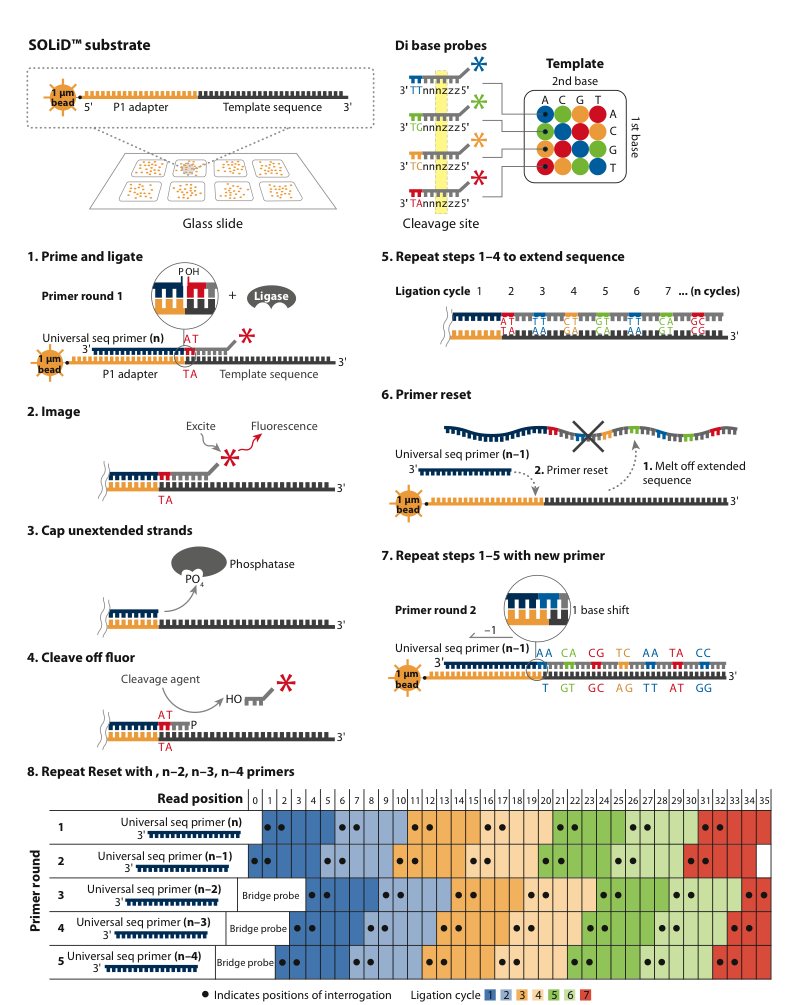
\includegraphics[width=0.7\linewidth]{solida}}
		\caption{Solid测序技术}
		\label{fig:solida}
	\end{figure}
	
	\item[连接酶测序] \hfill \\
	这一步是Solid测序的独特之处。它并没有采用以前测序时所常用的DNA聚合酶,而是采用了连接酶。Solid连接反应的底物是8碱基单链荧光探针混合物,这里将其简单表示为:3’-XXnnnzzz-5’。连接反应中,这些探针按照碱基互补规则与单链DNA模板链配对。探针的5’末端分别标记了CY5、Texas Red、CY3、6-FAM这4种颜色的荧光染料, 如图\ref{fig:solida}。这个8碱基单链荧光探针中,第1和第2位碱基(XX)上的碱基是确定的,并根据种类的不同在6-8位(zzz)上加上了不同的荧光标记。这是Solid的独特测序法,两个碱基确定一个荧光信号,相当于一次能决定两个碱基。这种测序方法也称之为两碱基测序法。当荧光探针能够与DNA模板链配对而连接上时,就会发出代表第1,2位碱基的荧光信号,图\ref{fig:solida}和图\ref{fig:solidb}中的比色版所表示的是第1,2位碱基的不同组合与荧光颜色的关系。
	
			\begin{figure}[H] % Example image
		\center{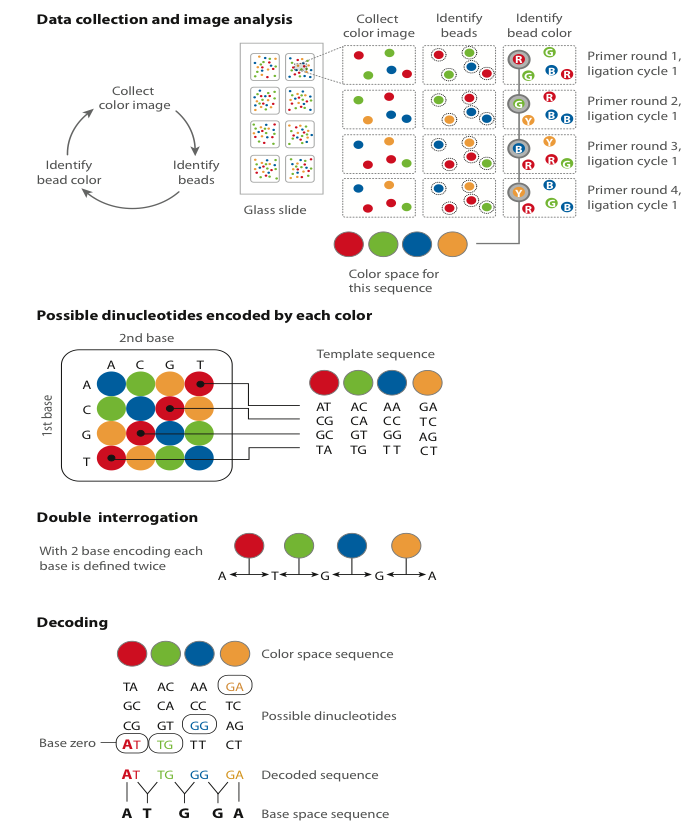
\includegraphics[width=0.7\linewidth]{solidb}}
		\caption{Solid测序技术}
		\label{fig:solidb}
	\end{figure}
	
	在记录下荧光信号后,通过化学方法在第5和第6位碱基之间进行切割,这样就能移除荧光信号,以便进行下一个位置的测序。不过值得注意的是,通过这种测序方法,每次测序的位置都相差5位。即第一次是第1、2位,第二次是第6、7位……在测到末尾后,要将新合成的链变性,洗脱。接着用引物n-1进行第二轮测序。引物n-1与引物n的区别是,二者在与接头配对的位置上相差一个碱基(图\ref{fig:solida}. 8)。也即是,通过引物n-1在引物n的基础上将测序位置往3’端移动一个碱基位置,因而就能测定第0、1位和第5、6位……第二轮测序完成,依此类推,直至第五轮测序,最终可以完成所有位置的碱基测序,并且每个位置的碱基均被检测了两次。该技术的读长在2×50bp,后续序列拼接同样比较复杂。由于双次检测,这一技术的原始测序准确性高达99.94\%,而15x覆盖率时的准确性更是达到了99.999\%,应该说是目前第二代测序技术中准确性最高的了。但在荧光解码阶段,鉴于其是双碱基确定一个荧光信号,因而一旦发生错误就容易产生连锁的解码错误。
\end{description}


%----------------------------------------------------------------------------------------
%	MAJOR SECTION 1
%----------------------------------------------------------------------------------------

\section{第三代测序技术}
第二代测序技术测序平台和测序成本,测序费用,花费时间,建库等实验技术难度,错误率以及读长(150-400bp),分析工作的体量,对于满足更高的科研需求和在医疗诊断中的普及都是不小的阻碍。其PCR过程带来的误差和偏好或成为其在医疗诊断大规模运用的阻碍。针对NGS在应用上的种种不足,二代技术本身的改良以及第三代以上世代的新测序技术发展是历史的必然。


PacBio 的SMRT\cite{Paper:Niedringhaus} 技术,LifeTechnologies 的 IonTorrent\cite{Paper:Rothberg} 半导体测序技术和 Oxford NanoporeTechnologies 纳米孔单分子测序技术为代表的第三代测序技术。与前两代相比,他们最大的特点就是单分子测序,测序过程无需进行PCR扩增。



%------------------------------------------------

\subsection{PacBio SMR} % Sub-section
PacBio的SMRT仍然运用边合成边测序的策略,但是其超强活性的DNA聚合酶是实现超长读长(~1000bp)的关键。反应在纳米管中进行,方便达到超高通量的目的。利用的是ZMW(零模波导孔)原理在超小的纳米孔中区别荧光信号的背景。其测序速度很快,每秒约10个dNTP。目前的问题在于测序的错误率太高(81\%~83\%),这也是大多数三代技术需要解决的共同问题。不过错误随机,几乎没有偏向性,为其通过矫正来减少错误率提供了可能。目前这个技术已经投入市场。
\subsection{Oxford Nanopre MinlON} % Sub-section
Nanopore的MinlON测序仪应用纳米孔单分子技术,这是一种基于电信号的测序技术,比起其他的光信号测序技术来说是一个革新。技术核心是一种特殊的内有分子接头的纳米孔,由蛋白质小孔嵌在人造膜上形成。膜两侧加上电压,使电流通过小孔。当不同的DNA碱基通过纳米孔时,其对电流的阻碍作用短暂地影响流过纳米孔的电流强度,不同碱基影响的程度不同,这种差异被灵敏的电子设备捕捉从而鉴定所通过的碱基种类。这种技术的优点很多,读长长(大约在几十kb,甚至100 kb),错误随机,而不是聚集在读取的两端,通量较高,该公司也在努力简化样品制备流程。理论上运用这个技术RNA也可以直接测序,还能检测到甲基化的胞嘧啶。不过不能实现理想的错误率控制,或成为其投入市场的阻碍。该公司在2016年12月刚完成其第一轮的一亿英镑的融资。
\subsection{LifeTechnologies IonTorrent} % Sub-section
IonTorrent 使用半导体芯片,在芯片的微孔中固定DNA链。依次加入AGCT的碱基,DNA合成时如果碱基可以结合到模板链则会释放一个氢离子。这个氢离子导致局部HP值发生变化。离子传感器检测到PH 变化后,便将化学信号转变为序列信息。而如果DNA 链有两个连续的相同碱基,则记录到的信号翻倍,从而将其识别。如果不匹配,则记录不到变化。这种技术由于不涉及荧光激发和拍照,则运行时间被大大缩减(仅数小时),无需激光光源,光学系统和照相系统,也不需要荧光标记,规避了这些环节带来的误差。但是其读长不算太长(200bp),并且当遭遇多个连续的相同碱基时,强烈的PH变化会带来误差。


%------------------------------------------------



\section{总结} % Major section
可以看出,第一代和第二代测序技术除了通量和成本上的差异之外,其测序核心原理(除Solid是边连接边测序之外)都是基于边合成边测序的思想。

第二代测序技术的优点是成本较之一代大大下降,通量大大提升。但缺点是所引入PCR过程会在一定程度上增加测序的错误率,并且具有系统偏向性,同时读长也比较短。

第三代测序技术是为了解决第二代所存在的缺点而开发的,它的根本特点是单分子测序,不需要任何PCR的过程。这是为了能有效避免因PCR偏向性而导致的系统错误,同时提高读长,并要保持二代技术的高通量,低成本的优点。

通过测序技术的发展,技术的壁垒不断的被打破,基因测序离普通人也越来越近了。比如,测序技术在医疗检测中的应用越来越深入。我们可以察觉,测序技术正逐渐融入我们的生活,近年来的精准医疗就是一个很好的例子。而相关的生物临床及基因数据的爆发,预示着生物大数据时代已经到来,随着技术的不断发展,我们能做的事情将超乎人们的想象。


%	BIBLIOGRAPHY
%----------------------------------------------------------------------------------------

\begin{thebibliography}{99} 
 \bibitem[1]{Paper:sanger}
 Sanger, F. and Nicklen, S.  (1977)
 \newblock DNA sequencing with chain-terminating 
 \newblock 74, 5463–5467.
 
  \bibitem[2]{Paper:Mardis}
 Mardis, E. R.  (2008)
 \newblock Next-generation DNA sequencing methods. Annual review of genomics and human genetics
 \newblock   9, 387–402 
 
 \bibitem[3]{Paper:Shendure}
Shendure, J. and Ji, H. Next-generation  (2008)
 \newblock DNA sequencing. Nature biotechnology
 \newblock   26, 1135–45
 
 \bibitem[4]{Paper:Mardi}
Mardis, E. R.  (2010)
\newblock Sequencing technologies - the next generation
\newblock \emph{Nature reviews. Genetics}
\newblock  11, 31–46

 \bibitem[5]{Paper:Niedringhaus}
Niedringhaus, T. P., Milanova, D., Kerby, M. B., Snyder, M. P. , Barron, A. E.  (2011)
 \newblock Landscape of Next-Generation Sequencing Technologies
 \newblock  4327–4341
 
 \bibitem[6]{Paper:Rothberg}
Rothberg, J. M. et al.  (2011)
 \newblock An integrated semiconductor device enabling non-optical genome sequencing
  \newblock \emph{Nature}
 \newblock 475, 348–52
 
\end{thebibliography}


\end{document}